% Distance to rho per baseline row of docs/ic/baselines.json (2026-10-15).
% Every value is copied from that file's "baselines" rows; each row is one
% experiment. Build: pdflatex baselines_gap.tex; pdftoppm -png -r 160 -singlefile baselines_gap.pdf baselines_gap
\documentclass[border=4pt]{standalone}
\usepackage{pgfplots}
\pgfplotsset{compat=1.17}
\begin{document}
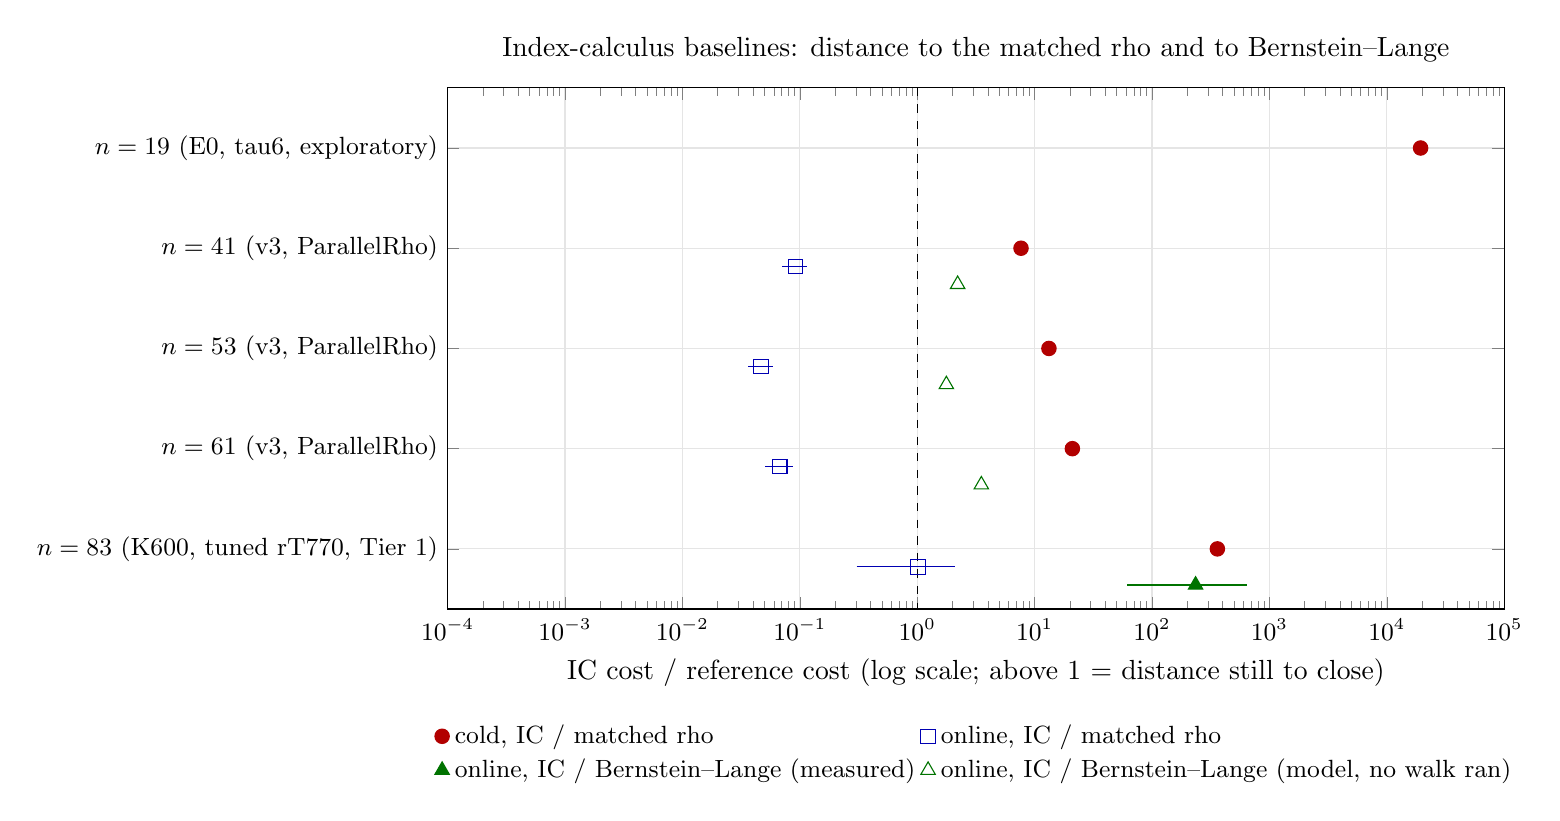
\begin{tikzpicture}
\begin{axis}[
  width=15cm, height=8.2cm,
  xmode=log, xmin=1e-4, xmax=1e5,
  ymin=0.4, ymax=5.6,
  ytick={1,2,3,4,5},
  yticklabels={
    {$n=19$ (E0, tau6, exploratory)},
    {$n=41$ (v3, ParallelRho)},
    {$n=53$ (v3, ParallelRho)},
    {$n=61$ (v3, ParallelRho)},
    {$n=83$ (K600, tuned rT770, Tier 1)}},
  y dir=reverse,
  xlabel={IC cost / reference cost (log scale; above 1 = distance still to close)},
  title={Index-calculus baselines: distance to the matched rho and to Bernstein--Lange},
  legend style={at={(0.5,-0.2)}, anchor=north, legend columns=2, font=\small, draw=none, cells={anchor=west}},
  grid=major, grid style={gray!20},
  tick label style={font=\small},
]
\addplot[black, dashed, forget plot] coordinates {(1,0.4) (1,5.6)};
\node[font=\scriptsize, anchor=south west] at (axis cs:1.1,0.45) {parity};

% cold gap IC/rho (95% intervals where the source gives one)
\addplot[only marks, mark=*, mark size=2.6pt, color=red!70!black]
  coordinates {
    (19400,1)
    (7.657,2)
    (13.24,3)
    (20.97,4)
    (360.4,5)
  };
\addlegendentry{cold, IC / matched rho}
% intervals drawn explicitly (log axis): [lo, hi]
\addplot[red!70!black, forget plot] coordinates {(16900,1) (22300,1)};
\addplot[red!70!black, forget plot] coordinates {(6.900,2) (8.613,2)};
\addplot[red!70!black, forget plot] coordinates {(11.75,3) (15.01,3)};
\addplot[red!70!black, forget plot] coordinates {(18.60,4) (23.84,4)};

% online gap IC/rho
\addplot[only marks, mark=square, mark size=2.6pt, color=blue!70!black]
  coordinates {(0.0915,2.18) (0.0466,3.18) (0.0675,4.18) (1.0125,5.18)};
\addlegendentry{online, IC / matched rho}
\addplot[blue!70!black, forget plot] coordinates {(0.0706,2.18) (0.1159,2.18)};
\addplot[blue!70!black, forget plot] coordinates {(0.0362,3.18) (0.0593,3.18)};
\addplot[blue!70!black, forget plot] coordinates {(0.0506,4.18) (0.0882,4.18)};
\addplot[blue!70!black, forget plot] coordinates {(0.304,5.18) (2.116,5.18)};

% online IC / Bernstein-Lange: measured at n=83, a model elsewhere
\addplot[only marks, mark=triangle*, mark size=3pt, color=green!45!black]
  coordinates {(235.0,5.36)};
\addlegendentry{online, IC / Bernstein--Lange (measured)}
\addplot[green!45!black, forget plot] coordinates {(61.4,5.36) (644.8,5.36)};
\addplot[only marks, mark=triangle, mark size=3pt, color=green!45!black]
  coordinates {(2.209,2.36) (1.771,3.36) (3.517,4.36)};
\addlegendentry{online, IC / Bernstein--Lange (model, no walk ran)}
\end{axis}
\end{tikzpicture}
\end{document}
